\section{Preventivo}
Per facilitare la lettura delle seguenti tabelle, vengono utilizzate delle sigle 
per identificare i ruoli:
\begin{itemize}
\item \textbf{Re:} \textit{Responsabile};
\item \textbf{Ad:} \textit{Amministratore};
\item \textbf{An:} \textit{Analista};
\item \textbf{Pt:} \textit{Progettista};
\item \textbf{Pr:} \textit{Programmatore};
\item \textbf{Ve:} \textit{Verificatore}.
\end{itemize}
\noindent
Inoltre, se le ore ricoperte in un determinato ruolo fossero nulle, la cella 
presenterà il simbolo \textbf{-} per indicarne l'assenza. 

\subsection{Fase di Analisi}
\subsubsection{Prospetto orario}
In questa fase, ogni componente del gruppo rivestirà i seguenti ruoli:
\begin{table}[H]
				\centering\renewcommand{\arraystretch}{1.5}
				\caption{Distribuzione delle ore nel periodo di Analisi}
				\vspace{0.2cm}
                \begin{tabular}{c c c c c c c c}
                               
                \rowcolorhead
                 {\colorhead \textbf{Nominativo}} &
                 {\colorhead \textbf{Re}} & 
                 {\colorhead \textbf{Am}} & 
                 {\colorhead\textbf{An}} & 
                 {\colorhead \textbf{Pt}} & 
                 {\colorhead\textbf{Pr}} & 
                 {\colorhead \textbf{Ve}} & 
                 {\colorhead \textbf{Ore totali} }\\
				
                \rowcolorlight
                 {\colorbody Riccardo Basso} & {\colorbody 8} & 
                 {\colorbody 8} & {\colorbody 11} & {\colorbody 8} & 
                 {\colorbody -} & {\colorbody -} & {\colorbody 35} 
				\\
				
				\rowcolordark
                 {\colorbody Marco Dalla Bà} & {\colorbody 10} & 
                 {\colorbody -} & {\colorbody 12} & {\colorbody 5} & 
                 {\colorbody -} & {\colorbody 8} & {\colorbody 35} 
				\\	
				
				\rowcolorlight
                 {\colorbody Riccardo Dario} & {\colorbody -} & 
                 {\colorbody -} & {\colorbody 11} & {\colorbody 6} & 
                 {\colorbody -} & {\colorbody 18} & {\colorbody 35} 
				\\
				              
                \rowcolordark
                 {\colorbody Irina Hornoiu} & {\colorbody 10} & 
                 {\colorbody 7} & {\colorbody 10} & {\colorbody -} & 
                 {\colorbody -} & {\colorbody 8} & {\colorbody 35} 
				\\
				
				\rowcolorlight
                 {\colorbody Diba Meysamiazad} & {\colorbody -} & 
                 {\colorbody 10} & {\colorbody 12} & {\colorbody -} & 
                 {\colorbody -} & {\colorbody 13} & {\colorbody 35} 
				\\
				
				\rowcolordark
                 {\colorbody Andrea Pigatto} & {\colorbody 10} & 
                 {\colorbody -} & {\colorbody 15} & {\colorbody -} & 
                 {\colorbody -} & {\colorbody 10} & {\colorbody 35} 
				\\	
				
				\rowcolorlight
                 {\colorbody \textbf{Ore totali ruolo}} & {\colorbody 38} & 
                 {\colorbody 25} & {\colorbody 71} & {\colorbody 19} & 
                 {\colorbody -} & {\colorbody 57} & {\colorbody 210} 
				\\
                

                \end{tabular}
               
\end{table}
\pagebreak
I dati ottenuti si possono riassumere nel seguente istogramma:
\begin{figure}[H] 
			\centering 
			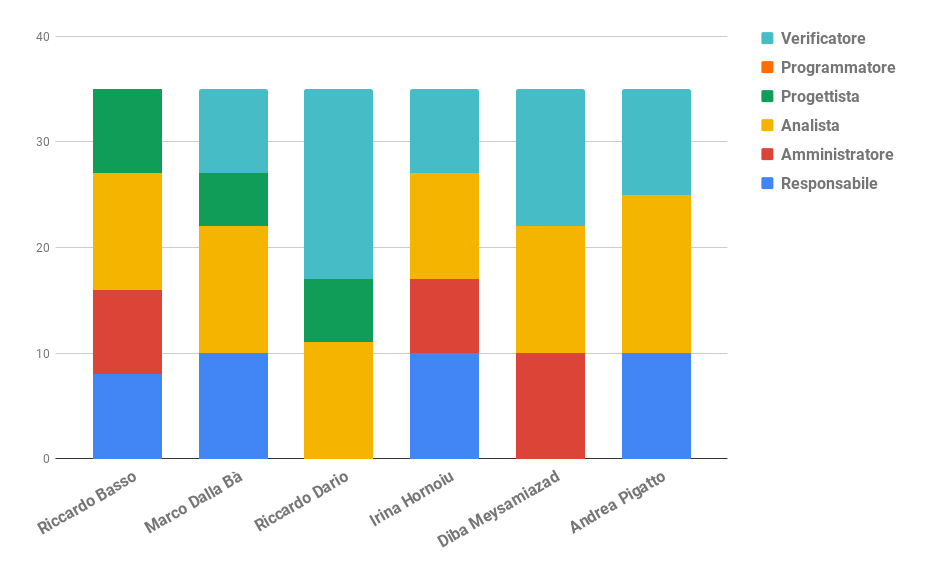
\includegraphics[width=0.9\textwidth]{res/images/istogramma_analisi.png}\\
				\caption{Istogramma della ripartizione di ore per ruolo in Analisi}
			\label{IstogrammaAnalisi}
\end{figure}


\subsubsection{Prospetto economico}
In questa fase il costo per ogni ruolo è il seguente:
\begin{table}[H]
	\centering\renewcommand{\arraystretch}{1.5}
	\caption{Prospetto dei costi per ruoli nel periodo di Analisi}
	\vspace{0.2cm}
    \begin{tabular}{c c c}
                   
    \rowcolorhead
     {\colorhead \textbf{Ruolo}} &
     {\colorhead \textbf{Ore}} & 
     {\colorhead \textbf{Costo}} \\
	
    \rowcolorlight
     {\colorbody Responsabile} & {\colorbody 38} & 
     {\colorbody \EUR{1.140,00}}  
	\\
	
	\rowcolordark
     {\colorbody Amministratore} & {\colorbody 25} & 
     {\colorbody \EUR{500,00}}
	\\	
	
	\rowcolorlight
     {\colorbody Analista} & {\colorbody 71} & 
     {\colorbody \EUR{1.775,00}} 
	\\
	
	\rowcolordark
     {\colorbody Progettista} & {\colorbody 19} & 
     {\colorbody \EUR{418,00}} 
	\\
	
	\rowcolorlight
     {\colorbody Programmatore} & {\colorbody -} & 
     {\colorbody -} 
	\\
	
	\rowcolordark
     {\colorbody Verificatore} & {\colorbody 57} & 
     {\colorbody \EUR{855,00}} 
	\\
	
	\rowcolorlight
     {\colorbody \textbf{Totale}} & {\colorbody 210} & 
     {\colorbody \EUR{4.688,00}} 
	
    \end{tabular} 
\end{table}
\pagebreak
I dati ottenuti si possono riassumere nel seguente areogramma:
\begin{figure}[H] 
\centering 
	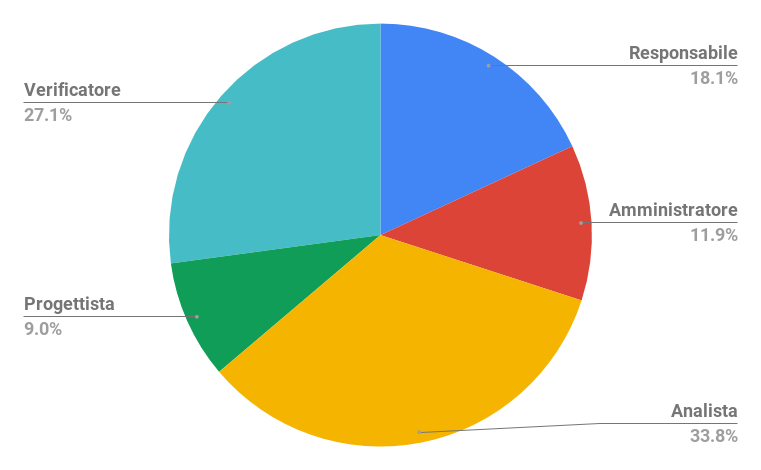
\includegraphics[width=0.7\textwidth]{res/images/areogramma_analisi.png}\\
	\caption{Areogramma della ripartizione di ore per ruolo in Analisi}
\label{AreogrammaAnalisi}
\end{figure}

\subsection{Fase di Consolidamento dei requisiti}
\subsubsection{Prospetto orario}
Il periodo di Consolidamento dei requisiti vede la seguente distribuzione oraria:
\begin{table}[H]
	\centering\renewcommand{\arraystretch}{1.5}
	\caption{Distribuzione delle ore nel periodo di Consolidamento 
		dei requisiti}
	\vspace{0.2cm}
    \begin{tabular}{c c c c c c c c}
                   
    \rowcolorhead
     {\colorhead \textbf{Nominativo}} &
     {\colorhead \textbf{Re}} & 
     {\colorhead \textbf{Am}} & 
     {\colorhead\textbf{An}} & 
     {\colorhead \textbf{Pt}} & 
     {\colorhead\textbf{Pr}} & 
     {\colorhead \textbf{Ve}} & 
     {\colorhead \textbf{Ore totali} }\\
	
    \rowcolorlight
     {\colorbody Riccardo Basso} & {\colorbody -} & 
     {\colorbody -} & {\colorbody 2} & {\colorbody -} & 
     {\colorbody -} & {\colorbody 3} & {\colorbody 5} 
	\\
	
	\rowcolordark
     {\colorbody Marco Dalla Bà} & {\colorbody 2} & 
     {\colorbody 3} & {\colorbody -} & {\colorbody -} & 
     {\colorbody -} & {\colorbody -} & {\colorbody 5} 
	\\	
	
	\rowcolorlight
     {\colorbody Riccardo Dario} & {\colorbody -} & 
     {\colorbody -} & {\colorbody 5} & {\colorbody -} & 
     {\colorbody -} & {\colorbody -} & {\colorbody 5} 
	\\
	
	\rowcolordark
     {\colorbody Irina Hornoiu} & {\colorbody -} & 
     {\colorbody -} & {\colorbody 5} & {\colorbody -} & 
     {\colorbody -} & {\colorbody -} & {\colorbody 5} 
	\\
    
    \rowcolorlight
     {\colorbody Diba Meysamiazad} & {\colorbody -} & 
     {\colorbody -} & {\colorbody -} & {\colorbody -} & 
     {\colorbody -} & {\colorbody 5} & {\colorbody 5} 
	\\
	
	\rowcolordark
     {\colorbody Andrea Pigatto} & {\colorbody 3} & 
     {\colorbody -} & {\colorbody -} & {\colorbody -} & 
     {\colorbody -} & {\colorbody 2} & {\colorbody 5} 
	\\	
	
	\rowcolorlight
     {\colorbody \textbf{Ore totali ruolo}} & {\colorbody 5} & 
     {\colorbody 3} & {\colorbody 12} & {\colorbody -} & 
     {\colorbody -} & {\colorbody 10} & { \colorbody 30} 
	\\

    \end{tabular}           
\end{table}
\pagebreak
I dati ottenuti si possono riassumere nel seguente istogramma:
\begin{figure}[H] 
			\centering 
				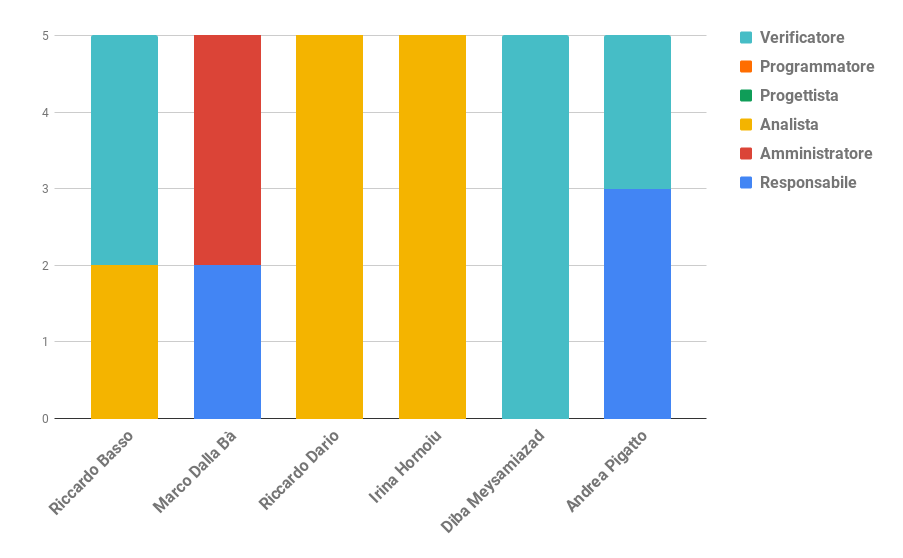
\includegraphics[width=0.9\textwidth]{res/images/istogramma_consolidamento.png}\\
				\caption{Istogramma della ripartizione di ore per ruolo in Consolidamento dei requisiti}
			\label{IstogrammaConsolidamento}
\end{figure}

\subsubsection{Prospetto economico}
In questa fase il costo per ogni ruolo è il seguente:
\begin{table}[H]
				\centering\renewcommand{\arraystretch}{1.5}
				\caption{Prospetto dei costi per ruoli nel periodo di 
					Consolidamento dei requisiti}
				\vspace{0.2cm}
                \begin{tabular}{c c c}
                               
                \rowcolorhead
                 {\colorhead \textbf{Ruolo}} &
                 {\colorhead \textbf{Ore}} & 
                 {\colorhead \textbf{Costo}} \\
				
                \rowcolorlight
                 {\colorbody Responsabile} & {\colorbody 5} & 
                 {\colorbody \EUR{150,00}}  
				\\
				
				\rowcolordark
                 {\colorbody Amministratore} & {\colorbody 3} & 
                 {\colorbody \EUR{60,00}}
				\\	
				
				\rowcolorlight
                 {\colorbody Analista} & {\colorbody 12} & 
                 {\colorbody \EUR{300,00}} 
				\\
				
				\rowcolordark
                 {\colorbody Progettista} & {\colorbody -} & 
                 {\colorbody -} 
				\\
				
				\rowcolorlight
                 {\colorbody Programmatore} & {\colorbody -} & 
                 {\colorbody -} 
				\\
				
				\rowcolordark
                 {\colorbody Verificatore} & {\colorbody 10} & 
                 {\colorbody \EUR{150,00}} 
				\\
				
				\rowcolorlight
                 {\colorbody \textbf{Totale}} & {\colorbody 30} & 
                 {\colorbody \EUR{660,00}} 
				\\
                

                \end{tabular}
                

\end{table}
\pagebreak
I dati ottenuti si possono riassumere nel seguente areogramma:
\begin{figure}[H] 
			\centering 
				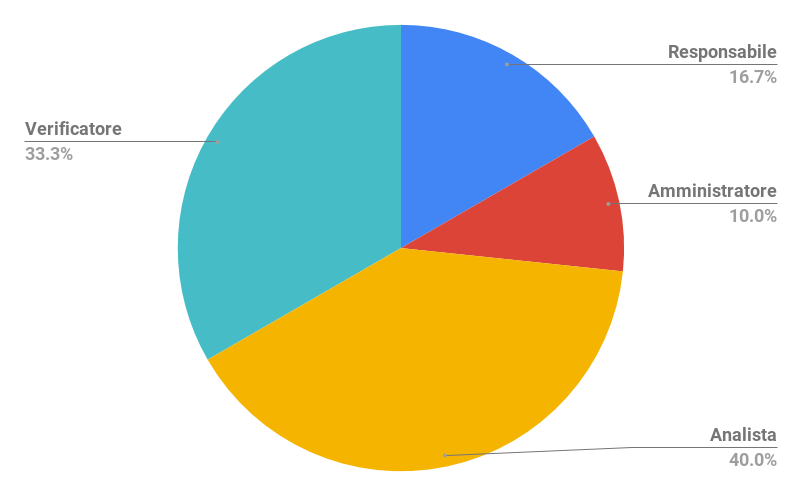
\includegraphics[width=0.7\textwidth]{res/images/areogramma_consolidamento.png}\\
				\caption{Areogramma della ripartizione di ore per ruolo in Consolidamento dei requisiti}
			\label{AreogrammaConsolidaemnto}
\end{figure}

\subsection{Fase di Progettazione architetturale}
\subsubsection{Prospetto orario}
Nella fase di Progettazione architetturale la distribuzione oraria è la seguente:
\begin{table}[H]
				\centering\renewcommand{\arraystretch}{1.5}
				\caption{Distribuzione delle ore nel periodo di Progettazione architetturale} 
				\vspace{0.2cm}
                \begin{tabular}{c c c c c c c c}
                              
                \rowcolorhead
                 {\colorhead \textbf{Nominativo}} &
                 {\colorhead \textbf{Re}} & 
                 {\colorhead \textbf{Am}} & 
                 {\colorhead\textbf{An}} & 
                 {\colorhead \textbf{Pt}} & 
                 {\colorhead\textbf{Pr}} & 
                 {\colorhead \textbf{Ve}} & 
                 {\colorhead \textbf{Ore totali} }\\
				
                \rowcolorlight
                 {\colorbody Riccardo Basso} & {\colorbody 6} & 
                 {\colorbody -} & {\colorbody 10} & {\colorbody -} & 
                 {\colorbody 6} & {\colorbody 6} & {\colorbody 28} 
				\\
				
				\rowcolordark
                 {\colorbody Marco Dalla Bà} & {\colorbody -} & 
                 {\colorbody -} & {\colorbody 5} & {\colorbody 8} & 
                 {\colorbody 5} & {\colorbody 10} & {\colorbody 28} 
				\\	
			
				\rowcolorlight
                 {\colorbody Riccardo Dario} & {\colorbody -} & 
                 {\colorbody 5} & {\colorbody -} & {\colorbody 7} & 
                 {\colorbody 6} & {\colorbody 10} & {\colorbody 28} 
				\\
					
				\rowcolordark
                 {\colorbody Irina Hornoiu} & {\colorbody -} & 
                 {\colorbody 5} & {\colorbody -} & {\colorbody 5} & 
                 {\colorbody 5} & {\colorbody 13} & {\colorbody 28} 
				\\
                
                \rowcolorlight
                 {\colorbody Diba Meysamiazad} & {\colorbody -} & 
                 {\colorbody 7} & {\colorbody 5} & {\colorbody 10} & 
                 {\colorbody -} & {\colorbody 6} & {\colorbody 28} 
				\\
				
				\rowcolordark
                 {\colorbody Andrea Pigatto} & {\colorbody 4} & 
                 {\colorbody -} & {\colorbody 9} & {\colorbody 11} & 
                 {\colorbody 4} & {\colorbody -} & {\colorbody 28} 
				\\	
				
				\rowcolorlight
                 {\colorbody \textbf{Ore totali ruolo}} & {\colorbody 10} & 
                 {\colorbody 17} & {\colorbody 29} & {\colorbody 41} & 
                 {\colorbody 26} & {\colorbody 45} & {\colorbody 168} 
				\\

                \end{tabular}             
\end{table}
\pagebreak
Una rappresentazione visiva della suddivisione oraria viene data dal seguente grafico:
\begin{figure}[H] 
			\centering 
				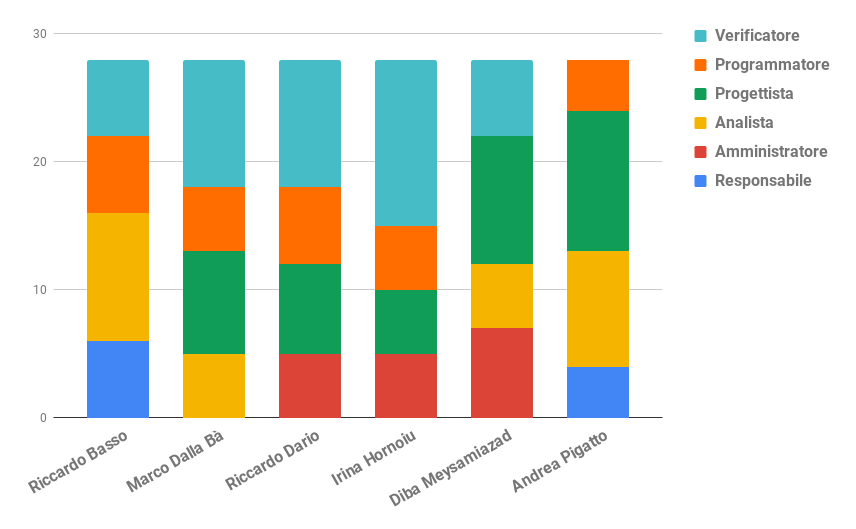
\includegraphics[width=0.9\textwidth]{res/images/istogramma_architetturale.png}\\
				\caption{Istogramma della ripartizione di ore per ruolo in Progettazione architetturale}
			\label{IstogrammaArchitetturale}
\end{figure}

\subsubsection{Prospetto economico}
In questa fase il costo per ogni ruolo è il seguente:
\begin{table}[H]
				\centering\renewcommand{\arraystretch}{1.5}
				\caption{Prospetto dei costi per ruoli nel periodo di 
					Progettazione architetturale}
				\vspace{0.2cm}
                \begin{tabular}{c c c}
                               
                \rowcolorhead
                 {\colorhead \textbf{Ruolo}} &
                 {\colorhead \textbf{Ore}} & 
                 {\colorhead \textbf{Costo}} \\
				
                \rowcolorlight
                 {\colorbody Responsabile} & {\colorbody 10} & 
                 {\colorbody \EUR{300,00}}  
				\\
				
				\rowcolordark
                 {\colorbody Amministratore} & {\colorbody 17} & 
                 {\colorbody \EUR{340,00}}
				\\	
				
				\rowcolorlight
                 {\colorbody Analista} & {\colorbody 29} & 
                 {\colorbody \EUR{725,00}} 
				\\
				
				\rowcolordark
                 {\colorbody Progettista} & {\colorbody 41} & 
                 {\colorbody \EUR{902,00}} 
				\\
				
				\rowcolorlight
                 {\colorbody Programmatore} & {\colorbody 26} & 
                 {\colorbody \EUR{390,00}} 
				\\
				
				\rowcolordark
                 {\colorbody Verificatore} & {\colorbody 45} & 
                 {\colorbody \EUR{675,00}} 
				\\
				
				\rowcolorlight
                 {\colorbody \textbf{Totale}} & {\colorbody 168} & 
                 {\colorbody \EUR{3.332,00}} 
				\\
                

                \end{tabular}
                

\end{table}
\pagebreak
I dati ottenuti si possono riassumere nel seguente areogramma:
\begin{figure}[H] 
			\centering 
				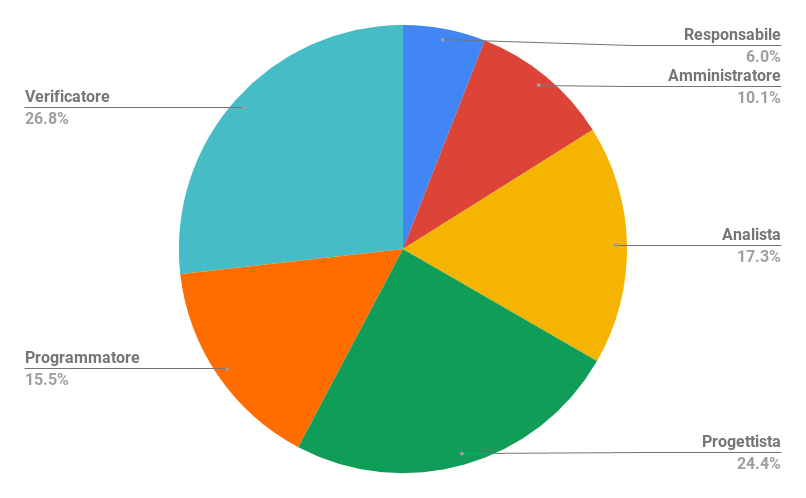
\includegraphics[width=0.7\textwidth]{res/images/areogramma_architetturale.png}\\
				\caption{Areogramma della ripartizione di ore per ruolo in Progettazione architetturale}
			\label{AreogrammaArchitetturale}
\end{figure}

\subsection{Fase di Progettazione di dettaglio e codifica}
\subsubsection{Prospetto orario}
Nella fase di Progettazione di dettaglio e codifica la distribuzione oraria è la seguente:
\begin{table}[H]
				\centering\renewcommand{\arraystretch}{1.5}
				\caption{Distribuzione delle ore nel periodo di Progettazione di dettaglio e codifica}
				\vspace{0.2cm}
                \begin{tabular}{c c c c c c c c}
                               
                \rowcolorhead
                 {\colorhead \textbf{Nominativo}} &
                 {\colorhead \textbf{Re}} & 
                 {\colorhead \textbf{Am}} & 
                 {\colorhead\textbf{An}} & 
                 {\colorhead \textbf{Pt}} & 
                 {\colorhead\textbf{Pr}} & 
                 {\colorhead \textbf{Ve}} & 
                 {\colorhead \textbf{Ore totali} }\\
				
                \rowcolorlight
                 {\colorbody Riccardo Basso} & {\colorbody -} & 
                 {\colorbody 8} & {\colorbody -} & {\colorbody 8} & 
                 {\colorbody 20} & {\colorbody 14} & {\colorbody 50} 
				\\
				
				\rowcolordark
                 {\colorbody Marco Dalla Bà} & {\colorbody 8} & 
                 {\colorbody 3} & {\colorbody -} & {\colorbody 6} & 
                 {\colorbody 20} & {\colorbody 13} & {\colorbody 50} 
				\\	
				
				\rowcolorlight
                 {\colorbody Riccardo Dario} & {\colorbody 4} & 
                 {\colorbody 4} & {\colorbody -} & {\colorbody 12} & 
                 {\colorbody 20} & {\colorbody 10} & {\colorbody 50} 
				\\
				
				\rowcolordark
                 {\colorbody Irina Hornoiu} & {\colorbody -} & 
                 {\colorbody -} & {\colorbody -} & {\colorbody 15} & 
                 {\colorbody 21} & {\colorbody 14} & {\colorbody 50} 
				\\
                
                \rowcolorlight
                 {\colorbody Diba Meysamiazad} & {\colorbody 4} & 
                 {\colorbody 6} & {\colorbody -} & {\colorbody 8} & 
                 {\colorbody 16} & {\colorbody 16} & {\colorbody 50} 
				\\
				
				\rowcolordark
                 {\colorbody Andrea Pigatto} & {\colorbody -} & 
                 {\colorbody -} & {\colorbody -} & {\colorbody 15} & 
                 {\colorbody 20} & {\colorbody 15} & {\colorbody 50} 
				\\	
				\rowcolorlight
                 {\colorbody \textbf{Ore totali ruolo}} & {\colorbody 16} & 
                 {\colorbody 21} & {\colorbody -} & {\colorbody 64} & 
                 {\colorbody 117} & {\colorbody 82} & {\colorbody 300} 
				\\

                \end{tabular}
                

\end{table}
\pagebreak
Una rappresentazione visiva della suddivisione oraria viene data dal seguente grafico:
\begin{figure}[H] 
			\centering 
				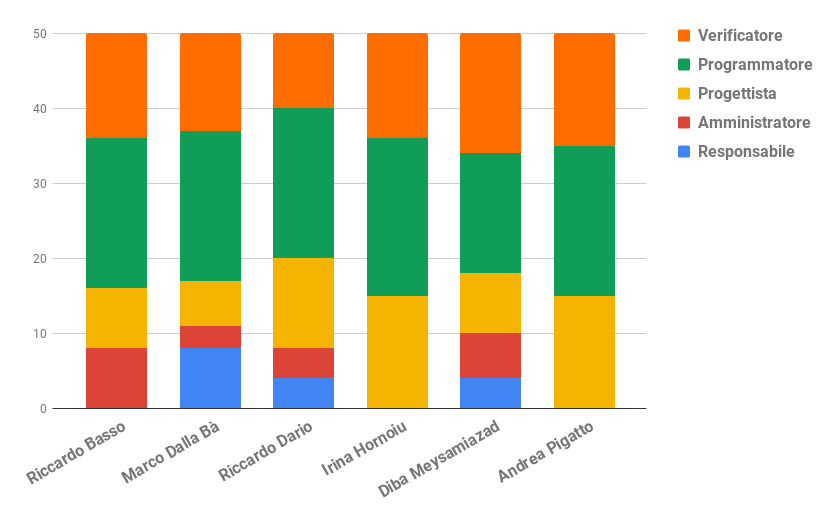
\includegraphics[width=0.9\textwidth]{res/images/istogramma_dettaglio.png}\\
				\caption{Istogramma della ripartizione di ore per ruolo in Progettazione di dettaglio e codifica}
			\label{IstogrammaDettaglio}
\end{figure}

\subsubsection{Prospetto economico}
In questa fase il costo per ogni ruolo è il seguente:
\begin{table}[H]
				\centering\renewcommand{\arraystretch}{1.5}
				\caption{Prospetto dei costi per ruoli nel periodo di 
					Progettazione di dettaglio e codifica}
				\vspace{0.2cm}
                \begin{tabular}{c c c}
                               
                \rowcolorhead
                 {\colorhead \textbf{Ruolo}} &
                 {\colorhead \textbf{Ore}} & 
                 {\colorhead \textbf{Costo}} \\
				
                \rowcolorlight
                 {\colorbody Responsabile} & {\colorbody 16} & 
                 {\colorbody \EUR{480,00}}  
				\\
				
				\rowcolordark
                 {\colorbody Amministratore} & {\colorbody 21} & 
                 {\colorbody \EUR{420,00}}
				\\	
				
				\rowcolorlight
                 {\colorbody Analista} & {\colorbody -} & 
                 {\colorbody -} 
				\\
				
				\rowcolordark
                 {\colorbody Progettista} & {\colorbody 64} & 
                 {\colorbody \EUR{1.408,00}} 
				\\
				
				\rowcolorlight
                 {\colorbody Programmatore} & {\colorbody 117} & 
                 {\colorbody \EUR{1.755,00}} 
				\\
				
				\rowcolordark
                 {\colorbody Verificatore} & {\colorbody 82} & 
                 {\colorbody \EUR{1.230,00}} 
				\\
				
				\rowcolorlight
                 {\colorbody \textbf{Totale}} & {\colorbody 300} & 
                 {\colorbody \EUR{5.293,00}} 
				\\
                

                \end{tabular}
                

\end{table}
\pagebreak
I dati ottenuti si possono riassumere nel seguente areogramma:
\begin{figure}[H] 
			\centering 
				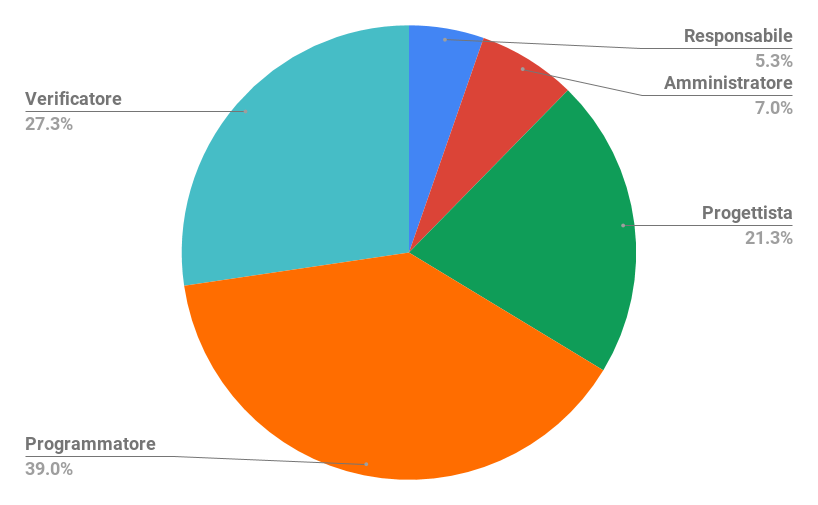
\includegraphics[width=0.7\textwidth]{res/images/areogramma_dettaglio.png}\\
				\caption{Areogramma della ripartizione di ore per ruolo in Progettazione di dettaglio e codifica}
			\label{AreogrammaDettaglio}
\end{figure}


\subsection{Fase di Validazione e collaudo}
\subsubsection{Prospetto orario}
Nella fase di progettazione di Validazione e collaudo la distribuzione oraria è la seguente:
\begin{table}[H]
				\centering\renewcommand{\arraystretch}{1.5}
				\caption{Distribuzione delle ore nel periodo di Validazione e 
					collaudo}
				\vspace{0.2cm}
                \begin{tabular}{c c c c c c c c}
                               
                \rowcolorhead
                 {\colorhead \textbf{Nominativo}} &
                 {\colorhead \textbf{Re}} & 
                 {\colorhead \textbf{Am}} & 
                 {\colorhead\textbf{An}} & 
                 {\colorhead \textbf{Pt}} & 
                 {\colorhead\textbf{Pr}} & 
                 {\colorhead \textbf{Ve}} & 
                 {\colorhead \textbf{Ore totali} }\\
				
                \rowcolorlight
                 {\colorbody Riccardo Basso} & {\colorbody -} & 
                 {\colorbody -} & {\colorbody -} & {\colorbody 5} & 
                 {\colorbody 5} & {\colorbody 10} & {\colorbody 20} 
				\\
				
				\rowcolordark
                 {\colorbody Marco Dalla Bà} & {\colorbody -} & 
                 {\colorbody -} & {\colorbody -} & {\colorbody 4} & 
                 {\colorbody 6} & {\colorbody 10} & {\colorbody 20} 
				\\	
				
				\rowcolorlight
                 {\colorbody Riccardo Dario} & {\colorbody 4} & 
                 {\colorbody 5} & {\colorbody -} & {\colorbody -} & 
                 {\colorbody 5} & {\colorbody 6} & {\colorbody 20} 
				\\
				
				\rowcolordark
                 {\colorbody Irina Hornoiu} & {\colorbody 4} & 
                 {\colorbody -} & {\colorbody -} & {\colorbody -} & 
                 {\colorbody 4} & {\colorbody 12} & {\colorbody 20} 
				\\
                
                \rowcolorlight
                 {\colorbody Diba Meysamiazad} & {\colorbody 5} & 
                 {\colorbody -} & {\colorbody -} & {\colorbody -} & 
                 {\colorbody 7} & {\colorbody 8} & {\colorbody 20} 
				\\
				
				\rowcolordark
                 {\colorbody Andrea Pigatto} & {\colorbody -} & 
                 {\colorbody 6} & {\colorbody -} & {\colorbody -} & 
                 {\colorbody 8} & {\colorbody 6} & {\colorbody 20} 
				\\	
				
				\rowcolorlight
                 {\colorbody \textbf{Ore totali ruolo}} & {\colorbody 13} & 
                 {\colorbody 11} & {\colorbody -} & {\colorbody 9} & 
                 {\colorbody 35} & {\colorbody 52} & {\colorbody 120} 
				\\

                \end{tabular}
                
\end{table}
\pagebreak
Una rappresentazione visiva della suddivisione oraria viene data dal seguente grafico:
\begin{figure}[H] 
			\centering 
				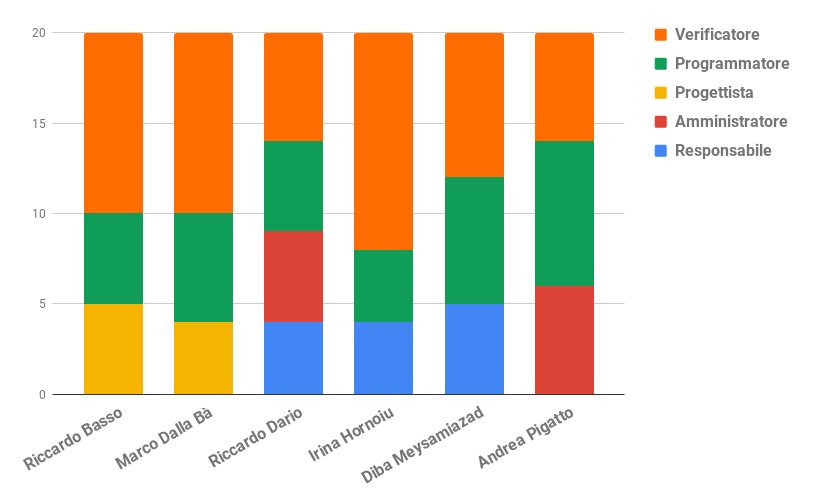
\includegraphics[width=0.9\textwidth]{res/images/istogramma_validazione.png}\\
				\caption{Istogramma della ripartizione di ore per ruolo in Validazione e collaudo}
			\label{IstogrammaValidazione}
\end{figure}

\subsubsection{Prospetto economico}
In questa fase il costo per ogni ruolo è il seguente:
\begin{table}[H]
				\centering\renewcommand{\arraystretch}{1.5}
				\caption{Prospetto dei costi per ruoli nel periodo di 
					Validazione e collaudo}
				\vspace{0.2cm}
                \begin{tabular}{c c c}
                               
                \rowcolorhead
                 {\colorhead \textbf{Ruolo}} &
                 {\colorhead \textbf{Ore}} & 
                 {\colorhead \textbf{Costo}} \\
				
                \rowcolorlight
                 {\colorbody Responsabile} & {\colorbody 13} & 
                 {\colorbody \EUR{390,00}}  
				\\
				
				\rowcolordark
                 {\colorbody Amministratore} & {\colorbody 11} & 
                 {\colorbody \EUR{220,00}}
				\\	
				
				\rowcolorlight
                 {\colorbody Analista} & {\colorbody -} & 
                 {\colorbody -} 
				\\
				
				\rowcolordark
                 {\colorbody Progettista} & {\colorbody 9} & 
                 {\colorbody \EUR{198,00}} 
				\\
				
				\rowcolorlight
                 {\colorbody Programmatore} & {\colorbody 35} & 
                 {\colorbody \EUR{525,00}} 
				\\
				
				\rowcolordark
                 {\colorbody Verificatore} & {\colorbody 52} & 
                 {\colorbody \EUR{780,00}} 
				\\
				
				\rowcolorlight
                 {\colorbody \textbf{Totale}} & {\colorbody 120} & 
                 {\colorbody \EUR{2.113,00}} 
				\\
                

                \end{tabular}
                

\end{table}
\pagebreak
I dati ottenuti si possono riassumere nel seguente areogramma:
\begin{figure}[H] 
			\centering 
				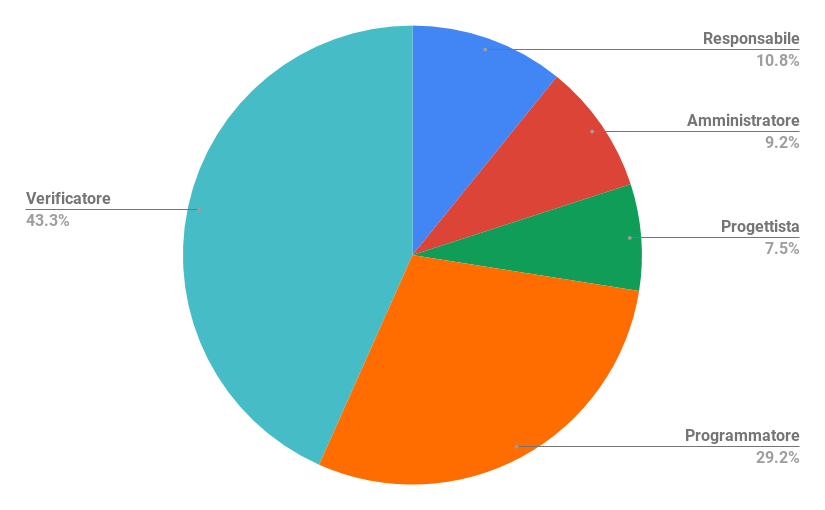
\includegraphics[width=0.7\textwidth]{res/images/areogramma_validazione.png}\\
				\caption{Areogramma della ripartizione di ore per ruolo in Validazione e collaudo}
			\label{AreogrammaValidazione}
\end{figure}


\subsection{Riepilogo}
\subsubsection{Ore totali}
\paragraph{Suddivisione del lavoro}\mbox{}\\
Vengono riportate il totale delle ore del progetto in cui sono presenti le ore di investimento e le ore rendicontate a carico del committente:
\begin{table}[H]
				\centering\renewcommand{\arraystretch}{1.5}
				\caption{Distribuzione delle ore totali di investimento e rendicontate}
				\vspace{0.2cm}
                \begin{tabular}{c c c c c c c c}
                               
                \rowcolorhead
                 {\colorhead \textbf{Nominativo}} &
                 {\colorhead \textbf{Re}} & 
                 {\colorhead \textbf{Am}} & 
                 {\colorhead\textbf{An}} & 
                 {\colorhead \textbf{Pt}} & 
                 {\colorhead\textbf{Pr}} & 
                 {\colorhead \textbf{Ve}} & 
                 {\colorhead \textbf{Ore totali} }\\
				
                \rowcolorlight
                 {\colorbody Riccardo Basso} & {\colorbody 14} & 
                 {\colorbody 16} & {\colorbody 23} & {\colorbody 21} & 
                 {\colorbody 31} & {\colorbody 33} & {\colorbody 138} 
				\\
				
				\rowcolordark
                 {\colorbody Marco Dalla Bà} & {\colorbody 20} & 
                 {\colorbody 6} & {\colorbody 17} & {\colorbody 23} & 
                 {\colorbody 31} & {\colorbody 41} & {\colorbody 138} 
				\\	
				
				\rowcolorlight
                 {\colorbody Riccardo Dario} & {\colorbody 8} & 
                 {\colorbody 14} & {\colorbody 16} & {\colorbody 25} & 
                 {\colorbody 31} & {\colorbody 44} & {\colorbody 138} 
				\\
				
				\rowcolordark
                 {\colorbody Irina Hornoiu} & {\colorbody 14} & 
                 {\colorbody 12} & {\colorbody 15} & {\colorbody 20} & 
                 {\colorbody 30} & {\colorbody 47} & {\colorbody 138} 
				\\
                
                \rowcolorlight
                 {\colorbody Diba Meysamiazad} & {\colorbody 9} & 
                 {\colorbody 23} & {\colorbody 17} & {\colorbody 18} & 
                 {\colorbody 23} & {\colorbody 48} & {\colorbody 138} 
				\\
				
				\rowcolordark
                 {\colorbody Andrea Pigatto} & {\colorbody 17} & 
                 {\colorbody 6} & {\colorbody 24} & {\colorbody 26} & 
                 {\colorbody 32} & {\colorbody 33} & {\colorbody 138} 
				\\	
				\rowcolorlight
                 {\colorbody \textbf{Ore totali ruolo}} & {\colorbody 82} & 
                 {\colorbody 77} & {\colorbody 112} & {\colorbody 133} & 
                 {\colorbody 178} & {\colorbody 246} & {\colorbody 828} 
				\\

                \end{tabular}
                

\end{table}
\pagebreak
Una rappresentazione visiva della suddivisione oraria viene data dal seguente grafico:
\begin{figure}[H] 
			\centering 
				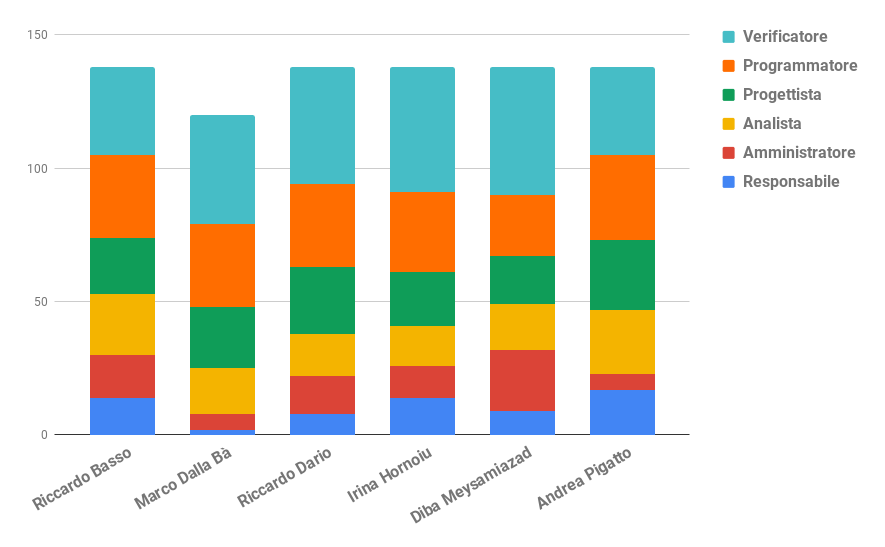
\includegraphics[width=0.9\textwidth]{res/images/istogramma_riepilogo.png}\\
				\caption{Istogramma della ripartizione di ore totali di investimento e rendicontate}
			\label{IstogrammaRiepilogo}
\end{figure}

\paragraph{Prospetto economico}\mbox{}\\
In questa fase il costo per ogni ruolo è il seguente:
\begin{table}[H]
				\centering\renewcommand{\arraystretch}{1.5}
				\caption{Prospetto dei costi totale delle ore di investimento e rendicontate}
				\vspace{0.2cm}
                \begin{tabular}{c c c}
                               
                \rowcolorhead
                 {\colorhead \textbf{Ruolo}} &
                 {\colorhead \textbf{Ore}} & 
                 {\colorhead \textbf{Costo}} \\
				
                \rowcolorlight
                 {\colorbody Responsabile} & {\colorbody 82} & 
                 {\colorbody \EUR{2.460,00}}  
				\\
				
				\rowcolordark
                 {\colorbody Amministratore} & {\colorbody 77} & 
                 {\colorbody \EUR{1.540,00}}
				\\	
				
				\rowcolorlight
                 {\colorbody Analista} & {\colorbody 112} & 
                 {\colorbody \EUR{2.800,00}} 
				\\
				
				\rowcolordark
                 {\colorbody Progettista} & {\colorbody 133} & 
                 {\colorbody \EUR{2.926,00}} 
				\\
				
				\rowcolorlight
                 {\colorbody Programmatore} & {\colorbody 178} & 
                 {\colorbody \EUR{2.670,00}} 
				\\
				
				\rowcolordark
                 {\colorbody Verificatore} & {\colorbody 246} & 
                 {\colorbody \EUR{3.690,00}} 
				\\
				
				\rowcolorlight
                 {\colorbody \textbf{Totale}} & {\colorbody 828} & 
                 {\colorbody \EUR{16.086,00}} 
				\\
                

                \end{tabular}
                

\end{table}
\pagebreak
I dati ottenuti si possono riassumere nel seguente areogramma:
\begin{figure}[H] 
			\centering 
				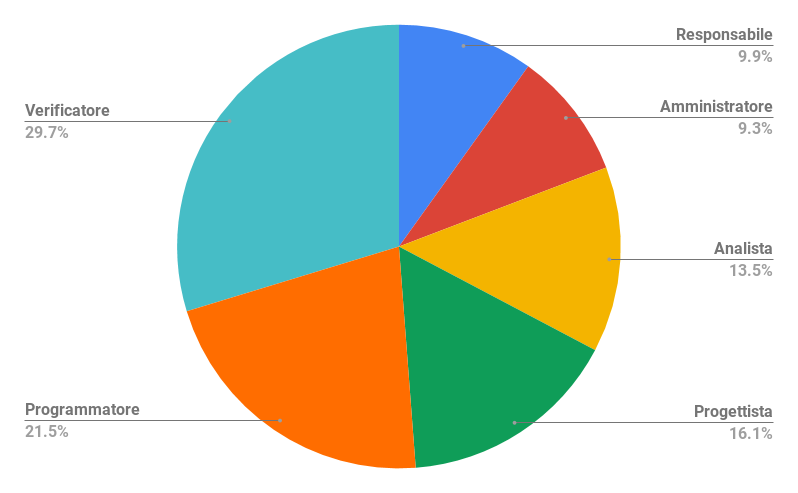
\includegraphics[width=0.7\textwidth]{res/images/areogramma_riepilogo.png}\\
				\caption{Areogramma dei costi totale delle ore di investimento e rendicontate}
			\label{AreogrammaRiepilogoRuoli}
\end{figure}


\subsubsection{Ore rendicontate}
\paragraph{Suddivisione del lavoro}\mbox{}\\
\linebreak
Le ore rendicontate sono riassunte nella seguente tabella:
\begin{table}[H]
				\centering\renewcommand{\arraystretch}{1.5}
				\caption{Distribuzione delle ore rendicontate}
				\vspace{0.2cm}
                \begin{tabular}{c c c c c c c c}
                               
                \rowcolorhead
                 {\colorhead \textbf{Nominativo}} &
                 {\colorhead \textbf{Re}} & 
                 {\colorhead \textbf{Am}} & 
                 {\colorhead\textbf{An}} & 
                 {\colorhead \textbf{Pt}} & 
                 {\colorhead\textbf{Pr}} & 
                 {\colorhead \textbf{Ve}} & 
                 {\colorhead \textbf{Ore totali} }\\
				
                \rowcolorlight
                 {\colorbody Riccardo Basso} & {\colorbody 8} & 
                 {\colorbody 10} & {\colorbody 15} & {\colorbody 11} & 
                 {\colorbody 29} & {\colorbody 30} & {\colorbody 103} 
				\\
				
				\rowcolordark
                 {\colorbody Marco Dalla Bà} & {\colorbody 15} & 
                 {\colorbody 2} & {\colorbody 11} & {\colorbody 15} & 
                 {\colorbody 25} & {\colorbody 35} & {\colorbody 103} 
				\\	
				
				\rowcolorlight
                 {\colorbody Riccardo Dario} & {\colorbody 5} & 
                 {\colorbody 11} & {\colorbody 10} & {\colorbody 19} & 
                 {\colorbody 29} & {\colorbody 29} & {\colorbody 103} 
				\\
				
				\rowcolordark
                 {\colorbody Irina Hornoiu} & {\colorbody 9} & 
                 {\colorbody 8} & {\colorbody 9} & {\colorbody 15} & 
                 {\colorbody 23} & {\colorbody 39} & {\colorbody 103} 
				\\
                
                \rowcolorlight
                 {\colorbody Diba Meysamiazad} & {\colorbody 6} & 
                 {\colorbody 16} & {\colorbody 10} & {\colorbody 12} & 
                 {\colorbody 19} & {\colorbody 40} & {\colorbody 103} 
				\\
				
				\rowcolordark
                 {\colorbody Andrea Pigatto} & {\colorbody 11} & 
                 {\colorbody 4} & {\colorbody 16} & {\colorbody 20} & 
                 {\colorbody 26} & {\colorbody 26} & {\colorbody 103} 
				\\	
				
				\rowcolorlight
                 {\colorbody \textbf{Ore totali ruolo}} & {\colorbody 54} & 
                 {\colorbody 51} & {\colorbody 71} & {\colorbody 92} & 
                 {\colorbody 151} & {\colorbody 199} & {\colorbody 618} 
				\\

                \end{tabular}
                

\end{table}

\begin{figure}[H] 
			\centering 
				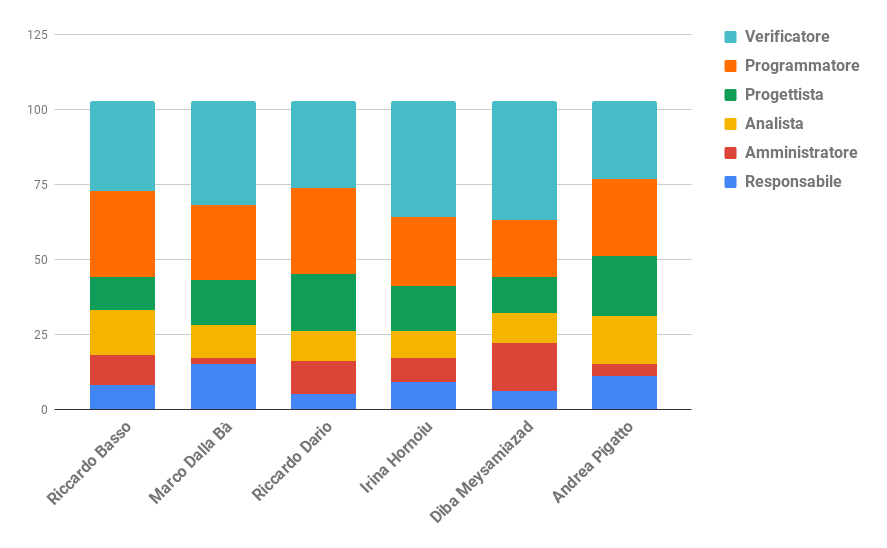
\includegraphics[width=0.9\textwidth]{res/images/istogramma_rendicontate.png}\\
				\caption{Istogramma della ripartizione delle ore rendicontate}
			\label{IstogrammaOreRendicontate}
\end{figure}

\paragraph{Prospetto economico}\mbox{}\\
\linebreak
Il totale rendicontato dei costi sostenuti per ogni ruolo è riassunto nella seguente tabella:

\begin{table}[H]
				\centering\renewcommand{\arraystretch}{1.5}
				\caption{Prospetto dei costi delle ore rendicontate}
				\vspace{0.2cm}
                \begin{tabular}{c c c}
                               
                \rowcolorhead
                 {\colorhead \textbf{Ruolo}} &
                 {\colorhead \textbf{Ore}} & 
                 {\colorhead \textbf{Costo}} \\
				
                \rowcolorlight
                 {\colorbody Responsabile} & {\colorbody 54} & 
                 {\colorbody \EUR{1.620,00}}  
				\\
				
				\rowcolordark
                 {\colorbody Amministratore} & {\colorbody 51} & 
                 {\colorbody \EUR{1.020,00}}
				\\	
				
				\rowcolorlight
                 {\colorbody Analista} & {\colorbody 71} & 
                 {\colorbody \EUR{1.775,00}} 
				\\
				
				\rowcolordark
                 {\colorbody Progettista} & {\colorbody 92} & 
                 {\colorbody \EUR{2.024,00}} 
				\\
				
				\rowcolorlight
                 {\colorbody Programmatore} & {\colorbody 151} & 
                 {\colorbody \EUR{2.265,00}} 
				\\
				
				\rowcolordark
                 {\colorbody Verificatore} & {\colorbody 199} & 
                 {\colorbody \EUR{2.985,00}} 
				\\
				
				\rowcolorlight
                 {\colorbody \textbf{Totale}} & {\colorbody 824} & 
                 {\colorbody \EUR{11.689,00}} 
				\\
                

                \end{tabular}
                

\end{table}
\pagebreak
I dati ottenuti si possono riassumere nel seguente areogramma:
\begin{figure}[H] 
			\centering 
				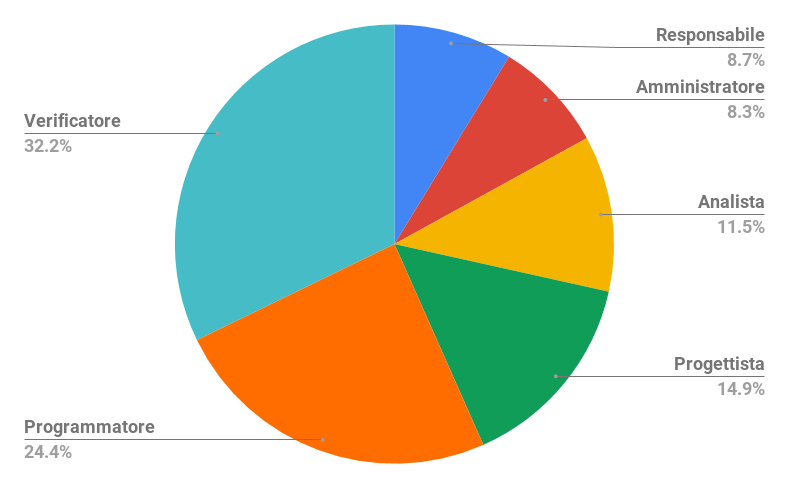
\includegraphics[width=0.7\textwidth]{res/images/areogramma_rendicontate.png}\\
				\caption{Areogramma delle ore rendicontate per ruolo}
			\label{AreogrammaOreRendicontate}
\end{figure}

\subsubsection{Conclusioni}
Il costo totale preventivato per il progetto è \EUR{11.689,00}.

